\section[几种典型跃迁]{几种典型跃迁} \label{sec:09.02} % 
% \makebox[5em][s]{} % 短题目拉间距

{\heiti 1.初、终态属于分立能谱,$H^{\prime}$为单频微扰}

设$t>0$时微扰$H^{\prime}$是单频的:
\begin{empheq}{align}\label{eq92.1}
	H^{\prime} &=\hat{F}(x)2\cos\omega_{0}t	\nonumber\\
	&=\hat{F}(x)(e^{i\omega_{0}t}+e^{-i\omega_{0}t})
\end{empheq}
其中$\hat{F}$为与时间无关的厄密算符.$(\hat{F}=\hat{F}^{+})$跃迁过程则完全按照$\S$\ref{sec:09.01}的提法,为了便于讨论,设终态能级片高于初态能级,即

微扰$H^{\prime}$的矩阵元为
\begin{empheq}{align}\label{eq92.2}
	H_{fk}^{\prime} &=\langle \varPsi_{f}|H^{\prime}|\varPsi_{k}\rangle \nonumber\\
	&=F_{fk}(e^{i\omega_{0}t}+e^{-i\omega_{0}t})
\end{empheq}
其中
\begin{empheq}{equation}\label{eq92.3}
	F_{fk}=\langle \varPsi_{f}|\hat{F}|\varPsi_{k}\rangle=\int\varPsi_{f}^{*}\hat{F}(x)\varPsi_{k}(x)dx
\end{empheq}
按照\eqref{eq91.12}式,容易求出
\eqindent{1}
\begin{empheq}{align}\label{eq92.4}
	C_{f}(t) &=\frac{F_{fk}}{i\hbar}\int_{0}^{t}(e^{i\omega_{0}t}+e^{-i\omega_{0}t})e^{i\omega_{fk}t}dt	\nonumber\\
	&=\frac{F_{fk}}{i\hbar}\left\{\frac{\exp[it(\omega_{fk}+\omega_{0})]-1}{i(\omega_{fk}+\omega_{0})}+\frac{\exp[it(\omega_{fk}-\omega_{0})]-1}{i(\omega_{fk}-\omega_{0})}\right\}
\end{empheq}\eqnormal
通常对跃迁概率进行测量的时刻,$H^{\prime}$已经作用了许多个周期,即总是满足条件$\omega_{0}t\gg2\pi$(以光波作用于原子为例,$\omega_{0}$约为$10^{15}\sim10^{16}\si{s^{-1}}$,当$t>10^{-13}\si{s}$,就满足这条件.)\eqref{eq92.4}式中分母为$(\omega_{fk}+\omega_{0})$的项可以略去,即取
\begin{empheq}{equation*}\label{eq92.4'}
	C_{f}(t)\approx\frac{F_{fk}}{\hbar}\cdot\frac{1-\exp[it(\omega_{fk}-\omega_{0})]}{\omega_{fk}-\omega_{0}}	\tag{$9.2.4^{\prime}$}
\end{empheq}
于是可得
\eqllong
\begin{empheq}{equation}\label{eq92.5}
	C_{f}^{*}(t)C_{f}(t)\approx\frac{|F_{fk}|^{2}}{\hbar^{2}}\frac{2}{(\omega_{fk}-\omega_{0})^{2}}[1-\cos(\omega_{fk}-\omega_{0})t]
\end{empheq}\eqnormal
跃迁速率为
\begin{empheq}{align}\label{eq92.6}
	w_{k\rightarrow f} &=\frac{d}{dt}[C_{f}^{*}(t)C_{f}(t)]	\nonumber\\
	&=\frac{2}{\hbar}|F_{fk}|^{2}\frac{\sin(\omega_{fk}-\omega_{0})t}{\omega_{fk}-\omega_{0}}
\end{empheq}
显然,仅当$\omega_{fk}\sim\omega_{0}$时,\eqref{eq92.6}式才有显著的值.利用公式
\begin{empheq}{equation}\label{eq92.7}
	\delta(x)=\frac{1}{2\pi}\int_{-\infty}^{\infty}e^{ikx}dk=\frac{\sin\alpha x}{\pi x}\quad (\alpha\rightarrow\infty)
\end{empheq}
可以对\eqref{eq92.6}式取下列近似
\begin{empheq}{equation}\label{eq92.8}
	\frac{\sin(\omega_{fk}-\omega_{0})t}{\pi(\omega_{fk}-\omega_{0})}\approx\delta(\omega_{fk}-\omega_{0})
\end{empheq}\eqlong
\begin{empheq}{align}\label{eq92.9}
	w_{k\rightarrow f}(t)\approx& \frac{2\pi}{\hbar^{2}}|F_{fk}|^{2}\delta(\omega_{fk}-\omega_{0})	\nonumber\\
	&=\frac{2\pi}{\hbar}|F_{fk}|^{2}\delta(E_{f}-E_{k}-\hbar\omega_{0})
\end{empheq}\eqnormal
其中$\delta$函数表明,仅当$(E_{f}-E_{k})=\hbar\omega_{0}$,跃迁速率才可能不为0,这正是能量守恒定律在跃迁过程中的具体体现.注意,跃迁速率$w_{k\rightarrow f}$与$t$无关(但必须以\eqref{eq92.8}式成立为前提),这时$C_{f}^{*}C_{f}$与$t$成正比,即
\eqshort
\begin{empheq}{equation}\label{eq92.10}
	C_{f}^{*}(t)C_{f}(t)\approx tw_{k\rightarrow f}
\end{empheq}\eqnormal
这表明$\varPsi_{k}\rightarrow\varPsi_{f}$跃迁过程在宏观时间尺度上是匀速进行的.

{\heiti 2.终态能级$E_{f}$属于连续能谱,$H^{\prime}$为单频微扰}

\begin{wrapfigure}[12]{r}{7em}
	\centering
	\small
	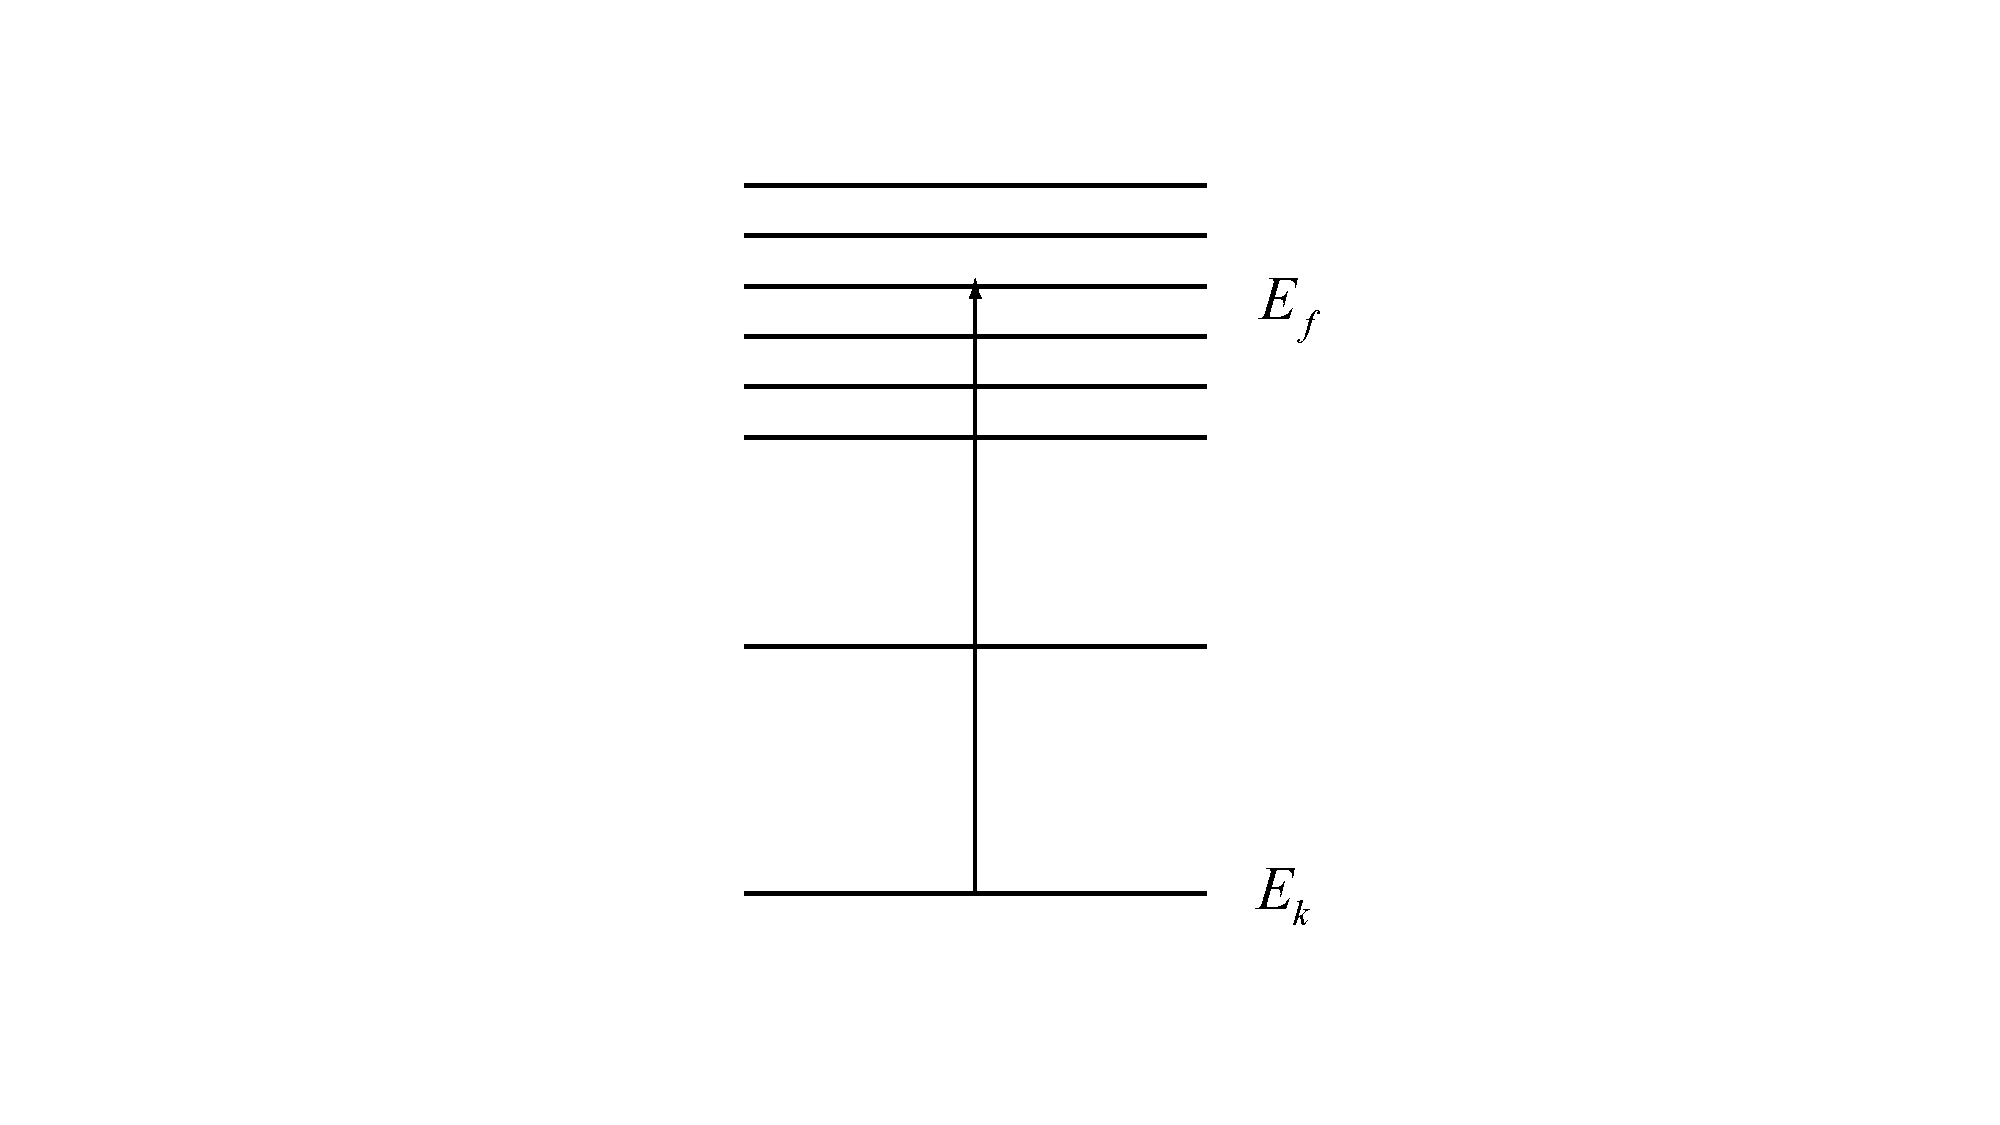
\includegraphics[width=3cm,clip]{QM file/figure/9-1}
	\caption{}\label{fig.9-1}
\end{wrapfigure}

仍设$H^{\prime}$为单频并取\eqref{eq92.1}式之形式.

连续能谱可以认为是能级密集的极限情形,如图\ref{fig.9-1}所示.由于终态能级密集,严格区分终态能量的微小差别既无可能,也无必要.有实际意义的做法是计算从初态$\varPsi_{k}$跃迁到能量接近$(E_{k}+\hbar\omega_{0})$的各个终态的概率总和.设在$E_{f}\approx(E_{k}+\hbar\omega_{0})$附近,能量范围$dE_{f}$内状态数为$\rho(E_{f})dE_{f}$,$\rho(E_{f})$称为状态密度.则由初态$\varPsi_{k}$向这些终态的跃迁速率总和为
\eqlong
\begin{equation}\label{eq92.11}
	W_{k\rightarrow f}=\int w_{k\rightarrow f}\rho(E_{f})dE_{f}
\end{equation}
将\eqref{eq92.9}式代入上式,得到
\begin{empheq}{equation}\label{eq92.12}
	\boxed{	W_{k\rightarrow f}=\frac{2\pi}{\hbar}|F_{fk}|^{2}\rho(E_{f}),\quad E_{f}=E_{k}+\hbar\omega_{0}	}
\end{empheq}\eqnormal
这公式有时称为黄金规则.在以上推导中假定$dE_{f}$范围内各个终态除能量略有差别外,其他方面的性质相同,特别是$F_{fk}$相同,这样由\eqref{eq92.11}式就得到\eqref{eq92.12}式.如果这些终态的$F_{fk}$有几种取值,则应按$F_{fk}$的数值将终态分类,对各类终态分别计算其状态密度和跃迁速率.

用紫外线(角频率$\omega_{0}$)照射原子,使原子中电子$(E_{k}<0)$电离$(E_{f}>0)$的过程(光电效应)就是属于本节讨论的问题.

{\heiti 3.常微扰}

设$t>0$时$H^{\prime}=H^{\prime}(x)$,与$t$无关这种情况相当于$\omega_{0}\rightarrow0$,只需在以上各公式中将$F_{fk}$换成$H_{fk}^{\prime}$,并取$\omega_{0}=0$就行了.例如\eqref{eq92.9}式改为
\begin{empheq}{equation}\label{eq92.13}
	w_{k\rightarrow f}\approx\frac{2\pi}{\hbar}|H_{fk}^{\prime}|^{2}\delta(E_{f}-E_{k})
\end{empheq}
其中$\delta$函数表明跃迁只能在能量相同的状态间发生.对于分立能级,常微扰将引起各简并态相互跃迁,结果导致这些简并态重新组合,形成新的定态.但如有某个简并态$\varPsi_{k}$,它与其他所有简并态(各$\varPsi_{f}$)之间$H_{fk}^{\prime}$均等于0,则$\varPsi_{k}$将不受微扰$H^{\prime}$的影响而保待其独立性,即在$H=H_{0}+H^{\prime}$的情况下,$\varPsi_{k}$仍是正确的定态波函数(在零级近似程度上,参看$\S$\ref{sec:06.02}).

\pskip
\example 弹性散射

按照量子跃迁的观点处理弹性散射,可以很便捷地导出散射截面的玻恩近似公式,如下.

\begin{figure}[!h]
	\centering
	\small
	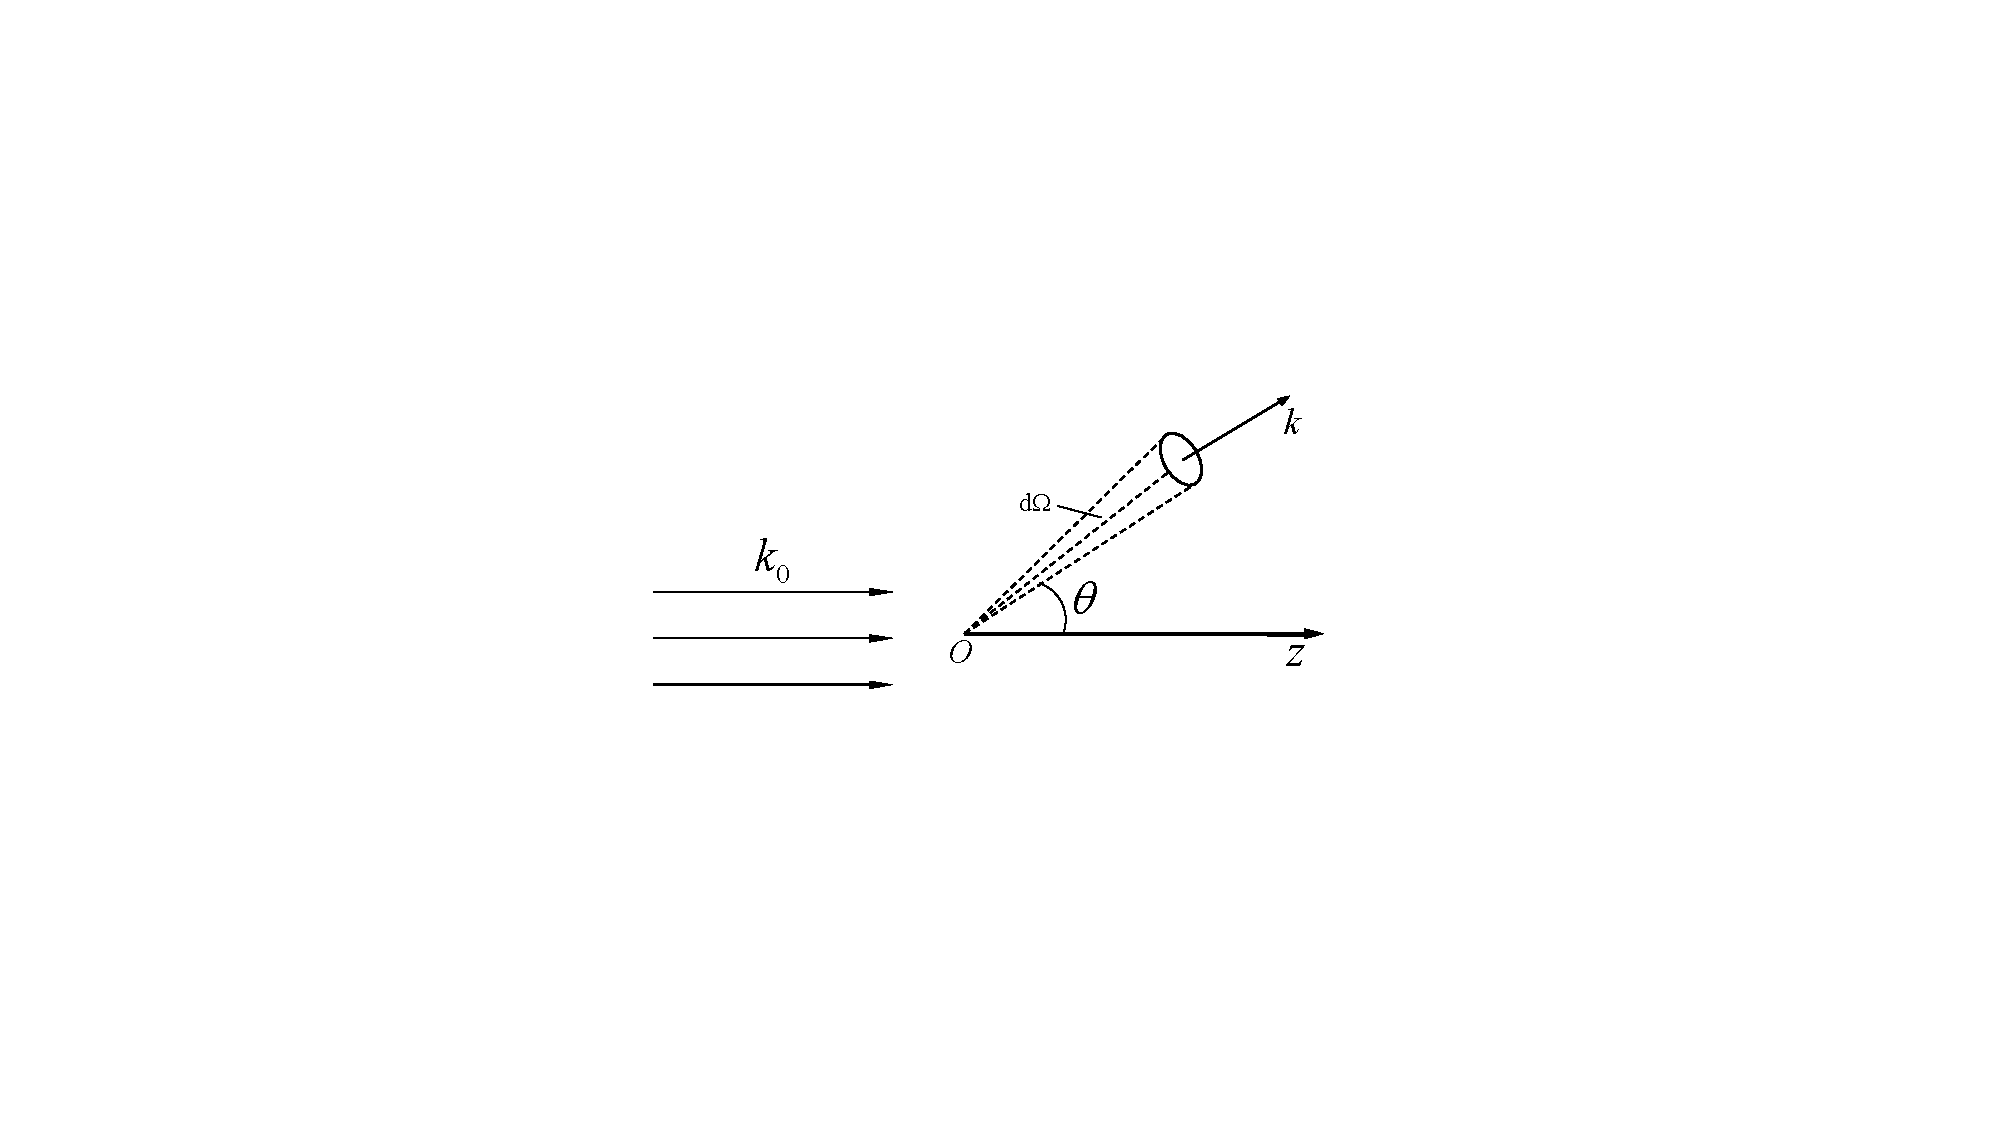
\includegraphics[width=6cm,clip]{QM file/figure/9-2}
	\caption{}\label{fig.9-2}
\end{figure}

散射过程中粒子的动量变化如图\ref{fig.9-2}所示.入射动量$\hbar k_{0}$,出射动量$\hbar k$,散射角$\theta$.为了便于计算状态密度,采用“箱归一化”方法($\S$\ref{sec:03.05}),“箱子”体积$L^{3}$.归一化的初态和终态波函数为
\begin{empheq}{align}
	\varPsi_{k_{0}}(\boldsymbol{r})=&L^{-\frac{3}{2}}e^{ik_{0}z}=L^{-\frac{3}{2}}e^{i\boldsymbol{k}_{0}\cdot\boldsymbol{r}}	\label{eq92.14}\\
	&\varPsi_{k}(\boldsymbol{r})=L^{-\frac{3}{2}}e^{i\boldsymbol{k}\cdot\boldsymbol{r}}	\label{eq92.15}
\end{empheq}
散射作用势视为常微扰,即令
\eqshort
\begin{empheq}{equation}\label{eq92.16}
	H^{\prime}=V(\boldsymbol{r})
\end{empheq}\eqnormal
在$V(\boldsymbol{r})$作用下粒子被散射到$(\theta,\varphi)$方向,相当于从初态$\varPsi_{k_{0}}$跃迁到终态$\varPsi_{k}$,由于终态动量$\hbar k$可以连续变化,应按连续谱处理,终态动量方向在$(\theta,\varphi)$附近$d\Omega$范围内的状态数为[参看\eqref{eq35.34}式]
\begin{empheq}{equation}\label{eq92.17}
	\rho(E)dE=\frac{L^{3}d^{3}\boldsymbol{p}}{h^{3}}=\frac{L^{3}\boldsymbol{p}^{2}dpd\Omega}{h^{3}}
\end{empheq}
终态动量与能量间有关系
\begin{empheq}{equation}\label{eq92.18}
	E=\frac{p^{2}}{2\mu},\quad dE=\frac{pdp}{\mu}
\end{empheq}
代入\eqref{eq92.17}式,即得
\begin{empheq}{equation}\label{eq92.19}
	\rho(E)=\frac{L^{3}\mu pd\Omega}{h^{3}}
\end{empheq}

由初态$\varPsi_{k_{0}}$跃迁到终态动量方向在$d\Omega$范围内的一切终态,跃迁速率总和可以按\eqref{eq92.12}式计算,即
\eqlong
\begin{empheq}{equation}\label{eq92.20}
	W=\frac{2\pi}{\hbar}|V_{kk_{0}}|^{2}\rho(E)=\frac{2\pi}{\hbar h^{3}}L^{3}\mu pd\omega|V_{kk_{0}}|^{2}
\end{empheq}\eqnormal
其中
\begin{empheq}{align}\label{eq92.21}
	V_{kk_{0}} &=\langle \varPsi_{k}|V|\varPsi_{k_{0}} \rangle 	\nonumber\\
	&=L^{-3}\int V(\boldsymbol{r})\exp[i(\boldsymbol{k_{0}}-\boldsymbol{k})\cdot\boldsymbol{r}]d^{3}\boldsymbol{r}
\end{empheq}

本题采用的“箱归一化”方法相当于体积$L^{3}$内有一个入射粒子,入射粒子流量为
\begin{empheq}{equation}\label{eq92.22}
	N_{0}=\frac{v}{L^{3}}=\frac{p}{\mu L^{3}}
\end{empheq}

单位时间内散射到$d\Omega$方向的粒子数$dN$应该就是由\eqref{eq92.20}式表示的跃迁速率和,即
\begin{empheq}{equation}\label{eq92.23}
	W=dN=N_{0}\sigma(\theta,\varphi)d\Omega
\end{empheq}
比较\eqref{eq92.20}、\eqref{eq92.22}、\eqref{eq92.23}式,即得微分散射截面公式.
\eqlong
\begin{empheq}{equation}\label{eq92.24}
	\sigma(\theta,\varphi)=\frac{\mu^{2}}{4\pi^{2}\hbar^{4}}\left|\int V(\boldsymbol{r})\exp[i(\boldsymbol{k_{0}}-\boldsymbol{k})\cdot\boldsymbol{r}]d^{3}\boldsymbol{r}\right|^{2}
\end{empheq}\eqnormal
这正是\eqref{eq84.32}式.$\S$\ref{sec:08.04}中$V(\boldsymbol{k},\boldsymbol{k_{0}})$相当于本题\eqref{eq92.21}式定义的$V_{kk_{0}}$乘以$L^{3}$.

如散射作用势$V$是中心力场,$V=V(r)$,则\eqref{eq92.21}中积分可以采用球坐标系,并以$(\boldsymbol{k_{0}}-\boldsymbol{k})$方向作为积分时的极轴,即令
\eqllong
\begin{empheq}{align*}
	&q=|\boldsymbol{k_{0}}-\boldsymbol{k}|,\quad (\boldsymbol{k_{0}}-\boldsymbol{k})\cdot\boldsymbol{r}=qr\cos\theta^{\prime}	\\
	\int V(r)\exp&[i(\boldsymbol{k_{0}}-\boldsymbol{k})\cdot\boldsymbol{r}]d^{3}\boldsymbol{r}=\int V(r)e^{iqr\cos\theta^{\prime}}r^{2}dr\sin\theta^{\prime}d\theta^{\prime}d\varphi^{\prime}
\end{empheq}\eqlong
其中角部积分可以算出,
\begin{empheq}{align}\label{eq92.25}
	\int e^{iqr\cos\theta^{\prime}}\sin\theta^{\prime}d\theta^{\prime}d\varphi^{\prime} &=2\pi\int_{0}^{\pi}e^{iqr\cos\theta^{\prime}}\sin\theta^{\prime}d\theta^{\prime}	\nonumber\\
	&=2\pi\int_{-1}^{1}e^{iqr\eta}d\eta=4\pi\frac{\sin qr}{qr}
\end{empheq}
因此
\begin{empheq}{equation}\label{eq92.26}
	\int V(r)\exp[i(\boldsymbol{k_{0}}-\boldsymbol{k})\cdot\boldsymbol{r}]d^{3}\boldsymbol{r}=\frac{4\pi}{q}\int_{0}^{\infty}\sin qrV(r)rdr
\end{empheq}\eqnormal
再代入\eqref{eq92.24}式,可求出$\sigma(\theta)$.\eqref{eq92.26}式中$q$是散射角$\theta$的函数,由图\ref{fig.9-2}可知
\begin{empheq}{equation}\label{eq92.27}
	q=|\boldsymbol{k_{0}}-\boldsymbol{k}|=2k\sin\left(\frac{\theta}{2}\right)
\end{empheq}


